\documentclass[11pt,letterpaper]{article}

\addtolength{\oddsidemargin}{-.875in}
\addtolength{\evensidemargin}{-.875in}
\addtolength{\textwidth}{1.75in}

\addtolength{\topmargin}{-.875in}
\addtolength{\textheight}{1.75in}

\usepackage[utf8]{inputenc}
\usepackage{caption} % for table captions
\usepackage{amsmath} % for multi-line equations and piecewises
\DeclareMathOperator{\sign}{sign}
\usepackage{graphicx}
\usepackage{relsize}
\usepackage{xspace}
\usepackage{verbatim} % for block comments
\usepackage{subcaption} % for subfigures
\usepackage{enumitem} % for a) b) c) lists
\usepackage{multirow}
\newcommand{\Cyclus}{\textsc{Cyclus}\xspace}%
\newcommand{\Cycamore}{\textsc{Cycamore}\xspace}%
\newcommand{\deploy}{\texttt{d3ploy}\xspace}%
\newcommand{\Deploy}{\texttt{D3ploy}\xspace}%
\usepackage{tabularx}
\usepackage{color}
\usepackage{multirow}
\usepackage{float} 
\usepackage[acronym,toc]{glossaries}
%\include{acros}
\definecolor{bg}{rgb}{0.95,0.95,0.95}
\newcolumntype{b}{X}
\newcolumntype{f}{>{\hsize=.15\hsize}X}
\newcolumntype{s}{>{\hsize=.5\hsize}X}
\newcolumntype{m}{>{\hsize=.75\hsize}X}
\newcolumntype{r}{>{\hsize=1.1\hsize}X}
\usepackage{titling}
\usepackage[hang,flushmargin]{footmisc}
\renewcommand*\footnoterule{}
\usepackage{tikz}

\usetikzlibrary{shapes.geometric,arrows}
\tikzstyle{process} = [rectangle, rounded corners, 
minimum width=1cm, minimum height=1cm,text centered, draw=black, 
fill=blue!30]
\tikzstyle{arrow} = [thick,->,>=stealth]

\graphicspath{}

\begin{document}

\section{1D-neutronics}

\subsection{1D-fuel}

	\begin{itemize}
		\item Mesh: \textit{1D-fuel.msh}
		\item Transient problem.
	\end{itemize}

Figure \ref{fig:1D-fuel} shows the results.

	\begin{figure}[htbp!]
		\centering
		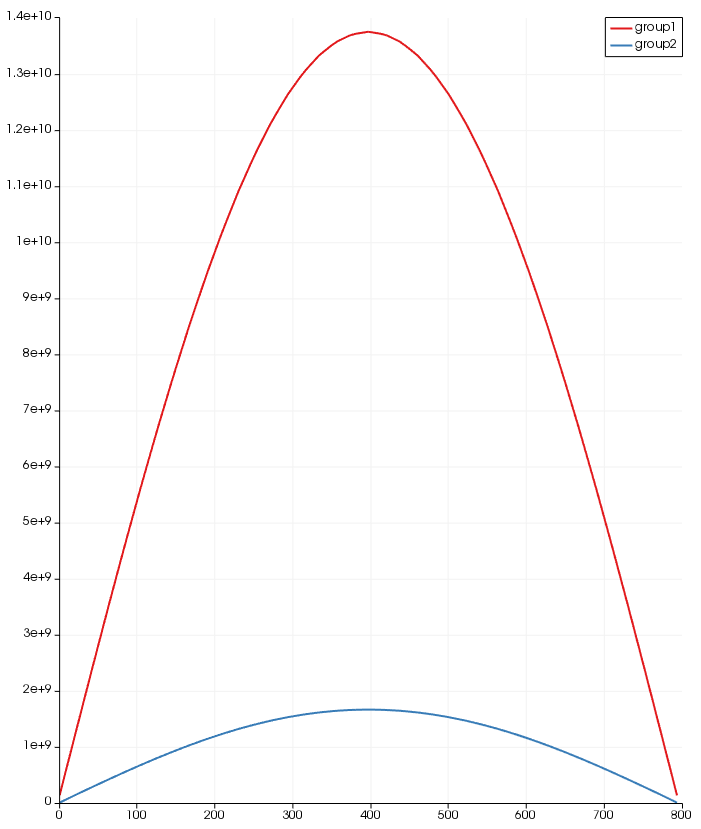
\includegraphics[height=5cm]{1D-fuel}
		\caption{Group 1 and 2 fluxes at 10 msec.}
		\label{fig:1D-fuel}
	\end{figure}

\subsection{1D-fuel-action}

	\begin{itemize}
		\item Mesh: GeneratedMesh
		\item Transient problem.
	\end{itemize}

Figure \ref{fig:1D-fuel-action} shows the results.

	\begin{figure}[htbp!]
		\centering
		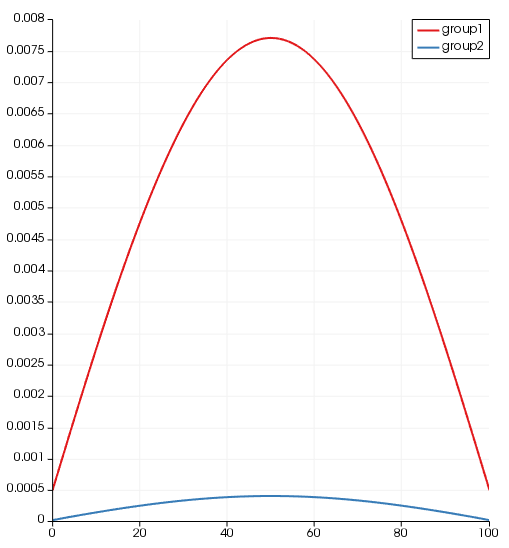
\includegraphics[height=5cm]{1D-fuel-action}
		\caption{Group 1 and 2 fluxes at 10 msec.}
		\label{fig:1D-fuel-action}
	\end{figure}

\subsection{1D-fuel-eig}

	\begin{itemize}
		\item Mesh: \textit{1D-fuel.msh}
		\item Eigenvalue problem: InversePowerMethod
	\end{itemize}

Figure \ref{fig:1D-fuel-eig} shows the results. 
FDM $k_{eff}$ = 1.415296. Both fluxes are normalized to the maximum value of the group 1 flux.
Moltres: $k_{eff}$ = 1.415418.

	\begin{figure}[htbp!]
		\centering
		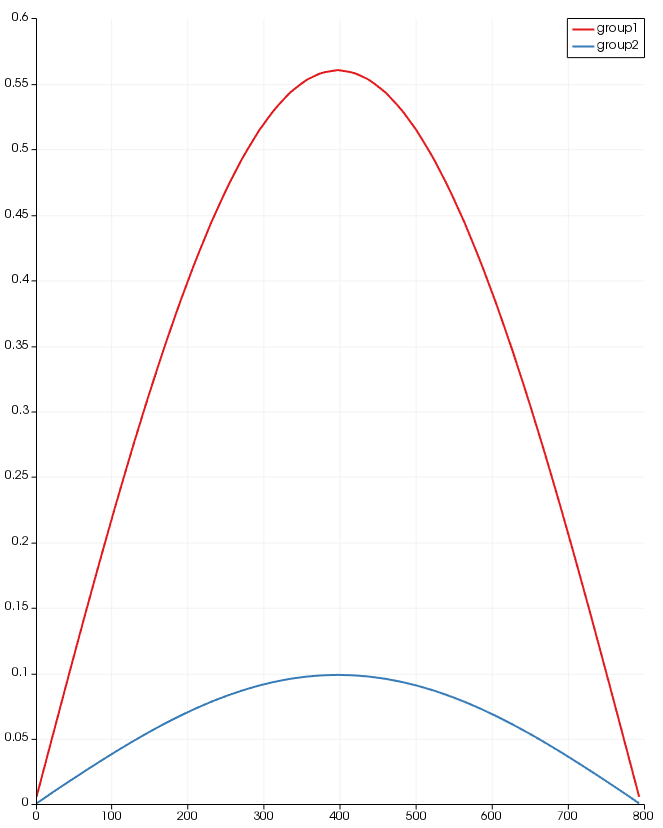
\includegraphics[height=5cm]{1D-fuel-eig}
		\caption{Steady state Group 1 and 2 fluxes.}
		\label{fig:1D-fuel-eig}
	\end{figure}

	\begin{figure}[htbp!]
		\centering
		\begin{subfigure}[t]{0.4\textwidth}
			\centering
			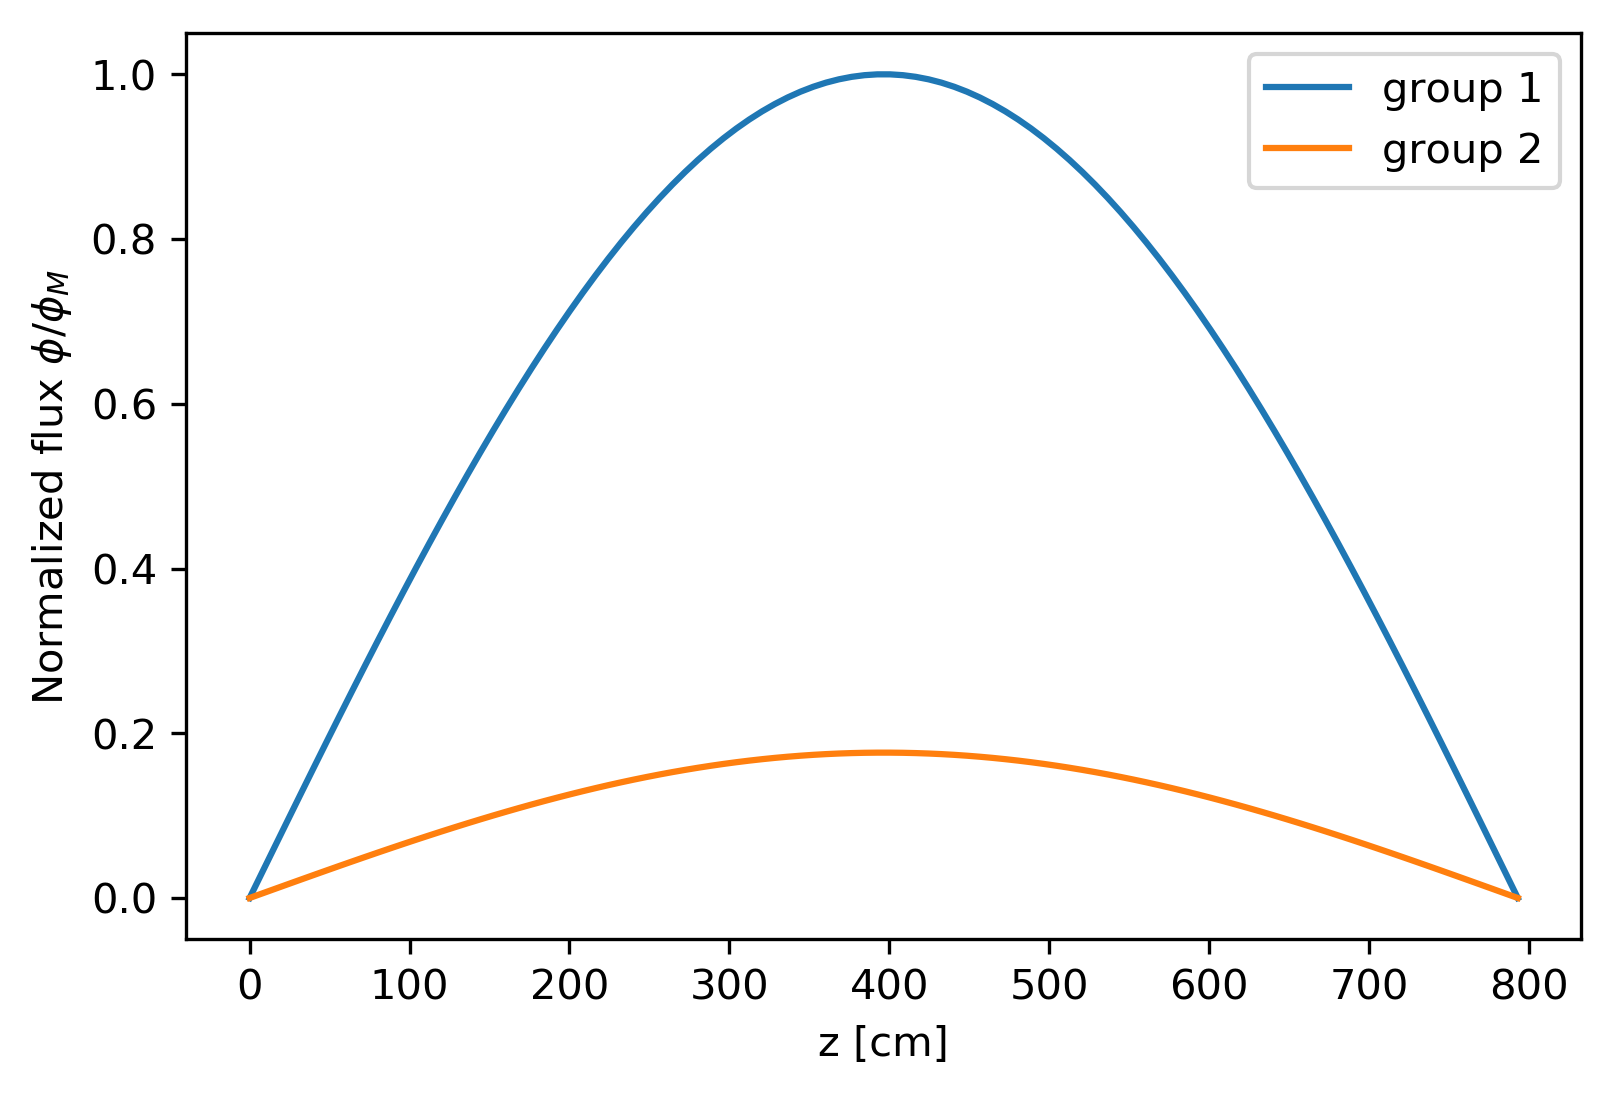
\includegraphics[width=\linewidth]{1D-fuel-eig-FDM}
			\caption{FDM.}
		\end{subfigure}
		\begin{subfigure}[t]{0.4\textwidth}
			\centering
			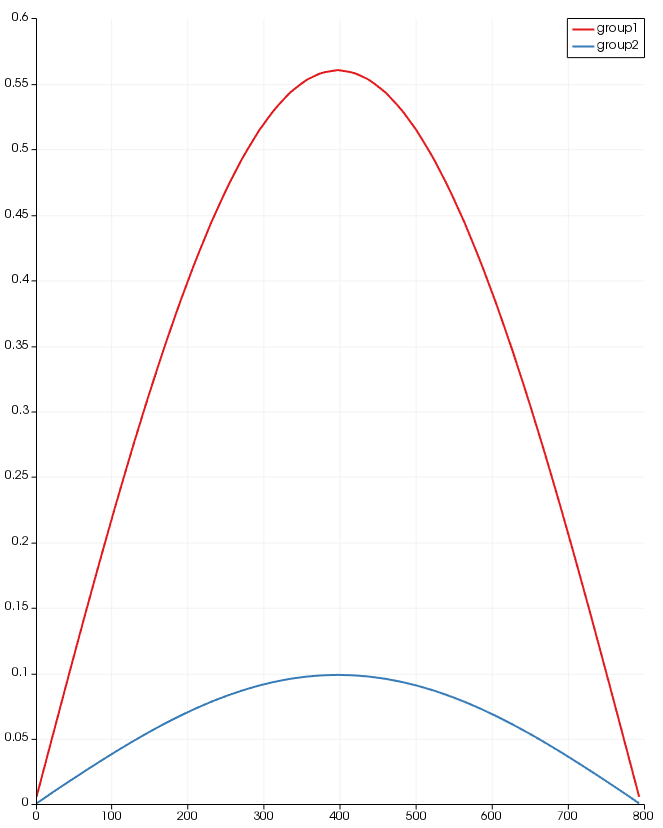
\includegraphics[width=\linewidth]{1D-fuel-eig}
			\caption{Moltres.}
		\end{subfigure}
		\hfill
		\caption{Steady state Group 1 and 2 fluxes.}
		\label{fig:1D-fuel-eig}
	\end{figure}

\subsection{1D-fuel-reflec}

	\begin{itemize}
		\item Mesh: \textit{1D-fuel-reflec.msh}
		\item Transient problem.
	\end{itemize}

Figure \ref{fig:1D-fuel-reflec} shows the results.

	\begin{figure}[htbp!]
		\centering
		\begin{subfigure}[t]{0.4\textwidth}
			\centering
			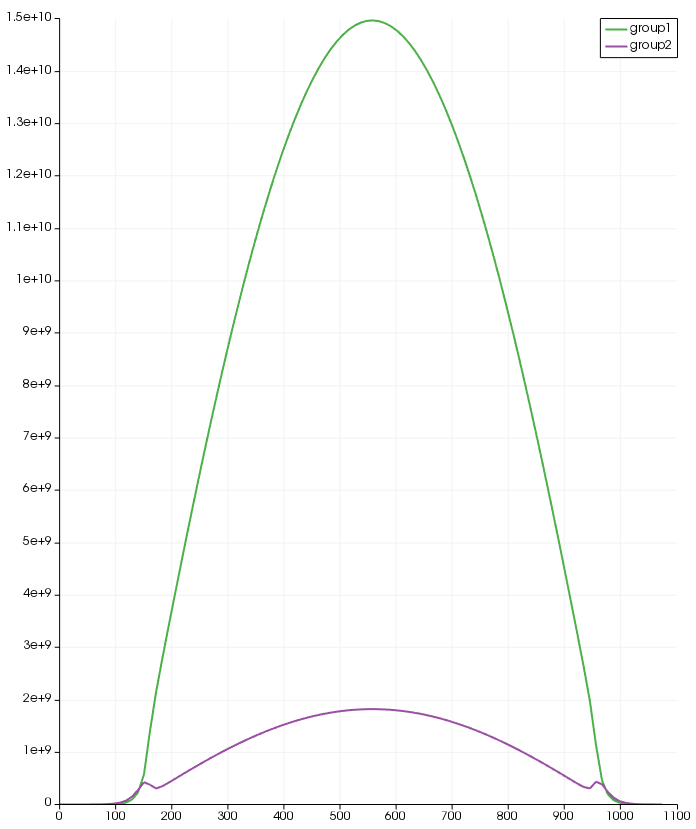
\includegraphics[width=\linewidth]{1D-fuel-reflec}
			\caption{Group 1 and 2 fluxes at 10 msec.}
		\end{subfigure}
		\begin{subfigure}[t]{0.4\textwidth}
			\centering
			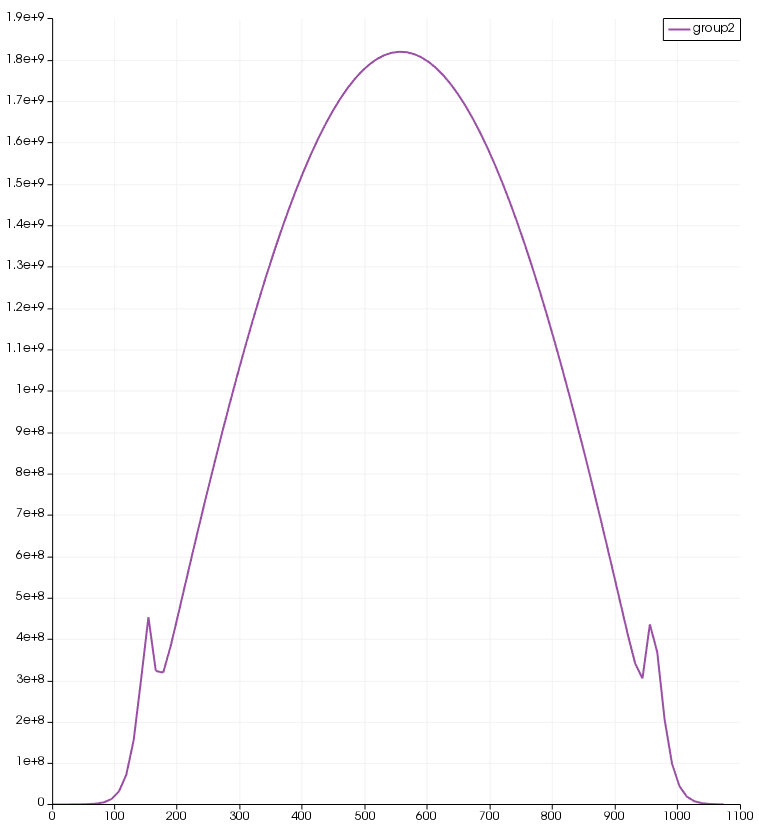
\includegraphics[width=\linewidth]{1D-fuel-reflec-g2}
			\caption{Group 2 flux at 10 msec.}
		\end{subfigure}
		\hfill
		\caption{Transient problem fluxes.}
		\label{fig:1D-fuel-reflec}
	\end{figure}

\subsection{1D-fuel-reflec-eig}

	\begin{itemize}
		\item Input files: \textit{1D-fuel-reflec-eig1.i} and \textit{1D-fuel-reflec-eig2.i}
		\item Mesh: \textit{1D-fuel-reflec.msh}
		\item Eigenvalue problem: InversePowerMethod and NonlinearEigen.
	\end{itemize}

Figures \ref{fig:1D-fuel-reflec-eig1} and \ref{fig:1D-fuel-reflec-eig2} show the results.
FDM $k_{eff}$ = 1.420210. Both fluxes are normalized to the maximum value of the group 1 flux.
Moltres: 
\begin{itemize}
	\item Inverse power method $k_{eff}$ = 1.424621.
	\item Non linear eigenvalue method $k_{eff}$ = 1.424644.
\end{itemize}

	\begin{figure}[htbp!]
		\centering
		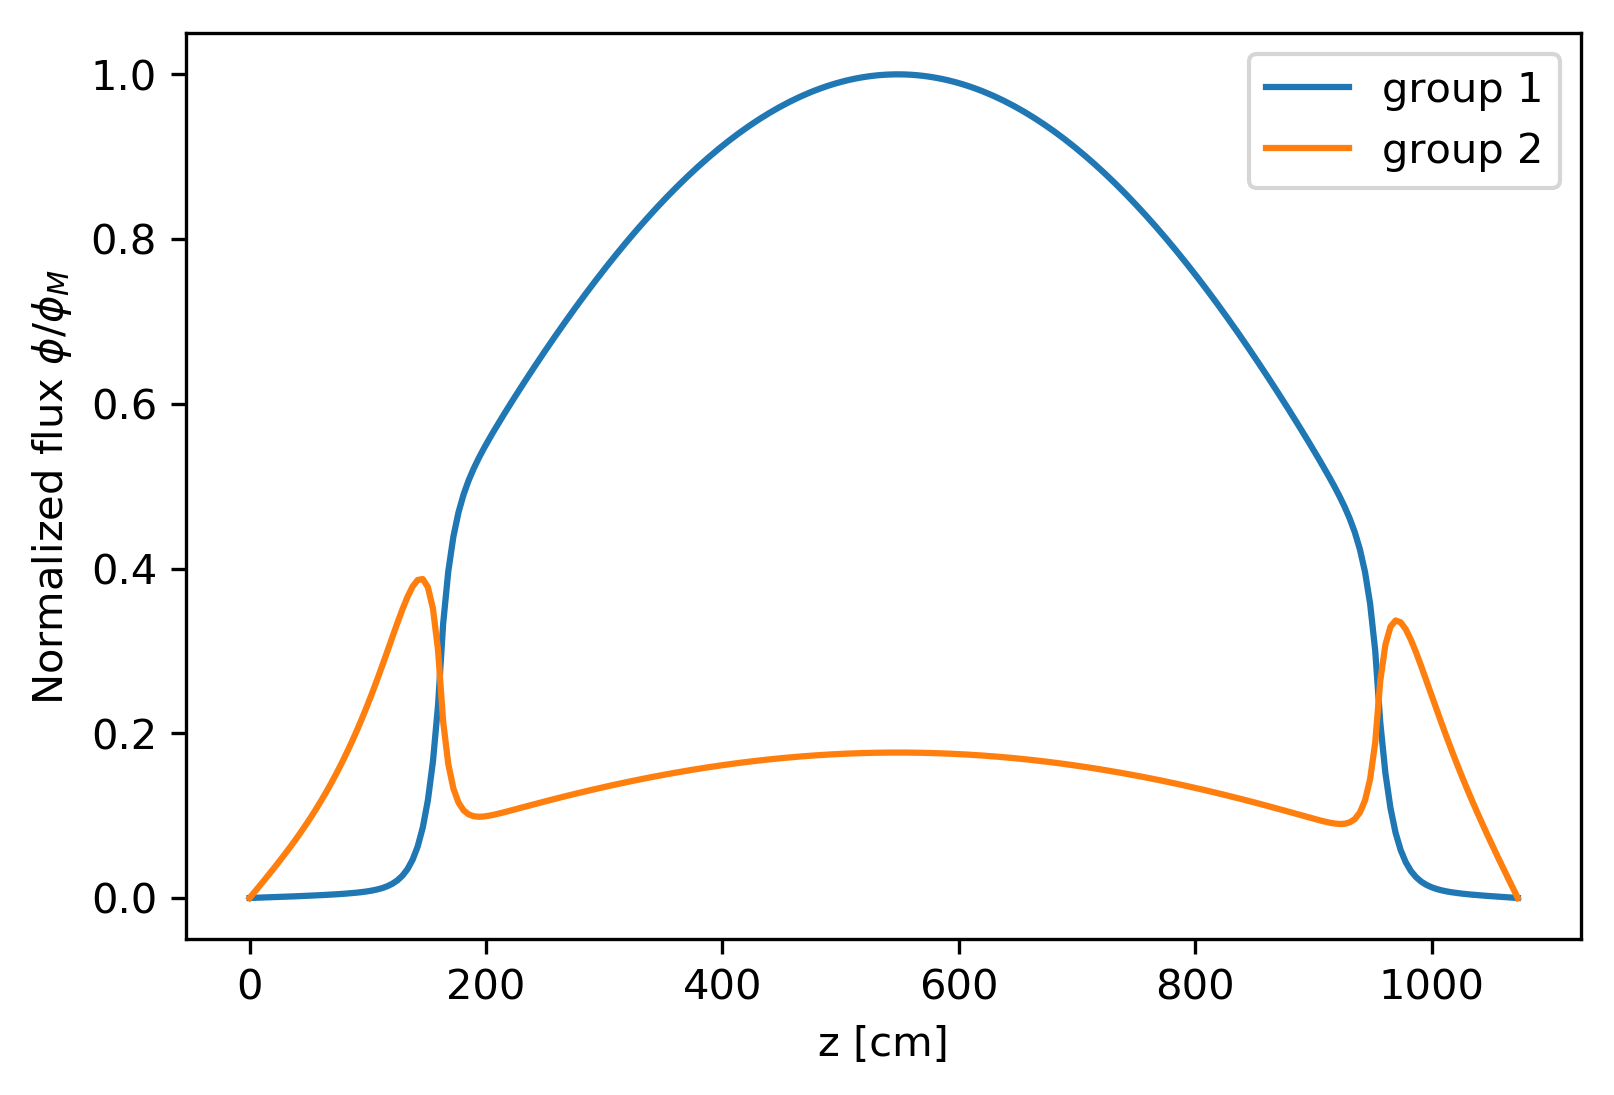
\includegraphics[height=5cm]{1D-fuel-reflec-eig-FDM}
		\caption{Steady state Group 1 and 2 fluxes using 1D FDM.}
		\label{fig:1D-fuel-reflec-eig1}
	\end{figure}

	\begin{figure}[htbp!]
		\centering
		\begin{subfigure}[t]{0.4\textwidth}
			\centering
			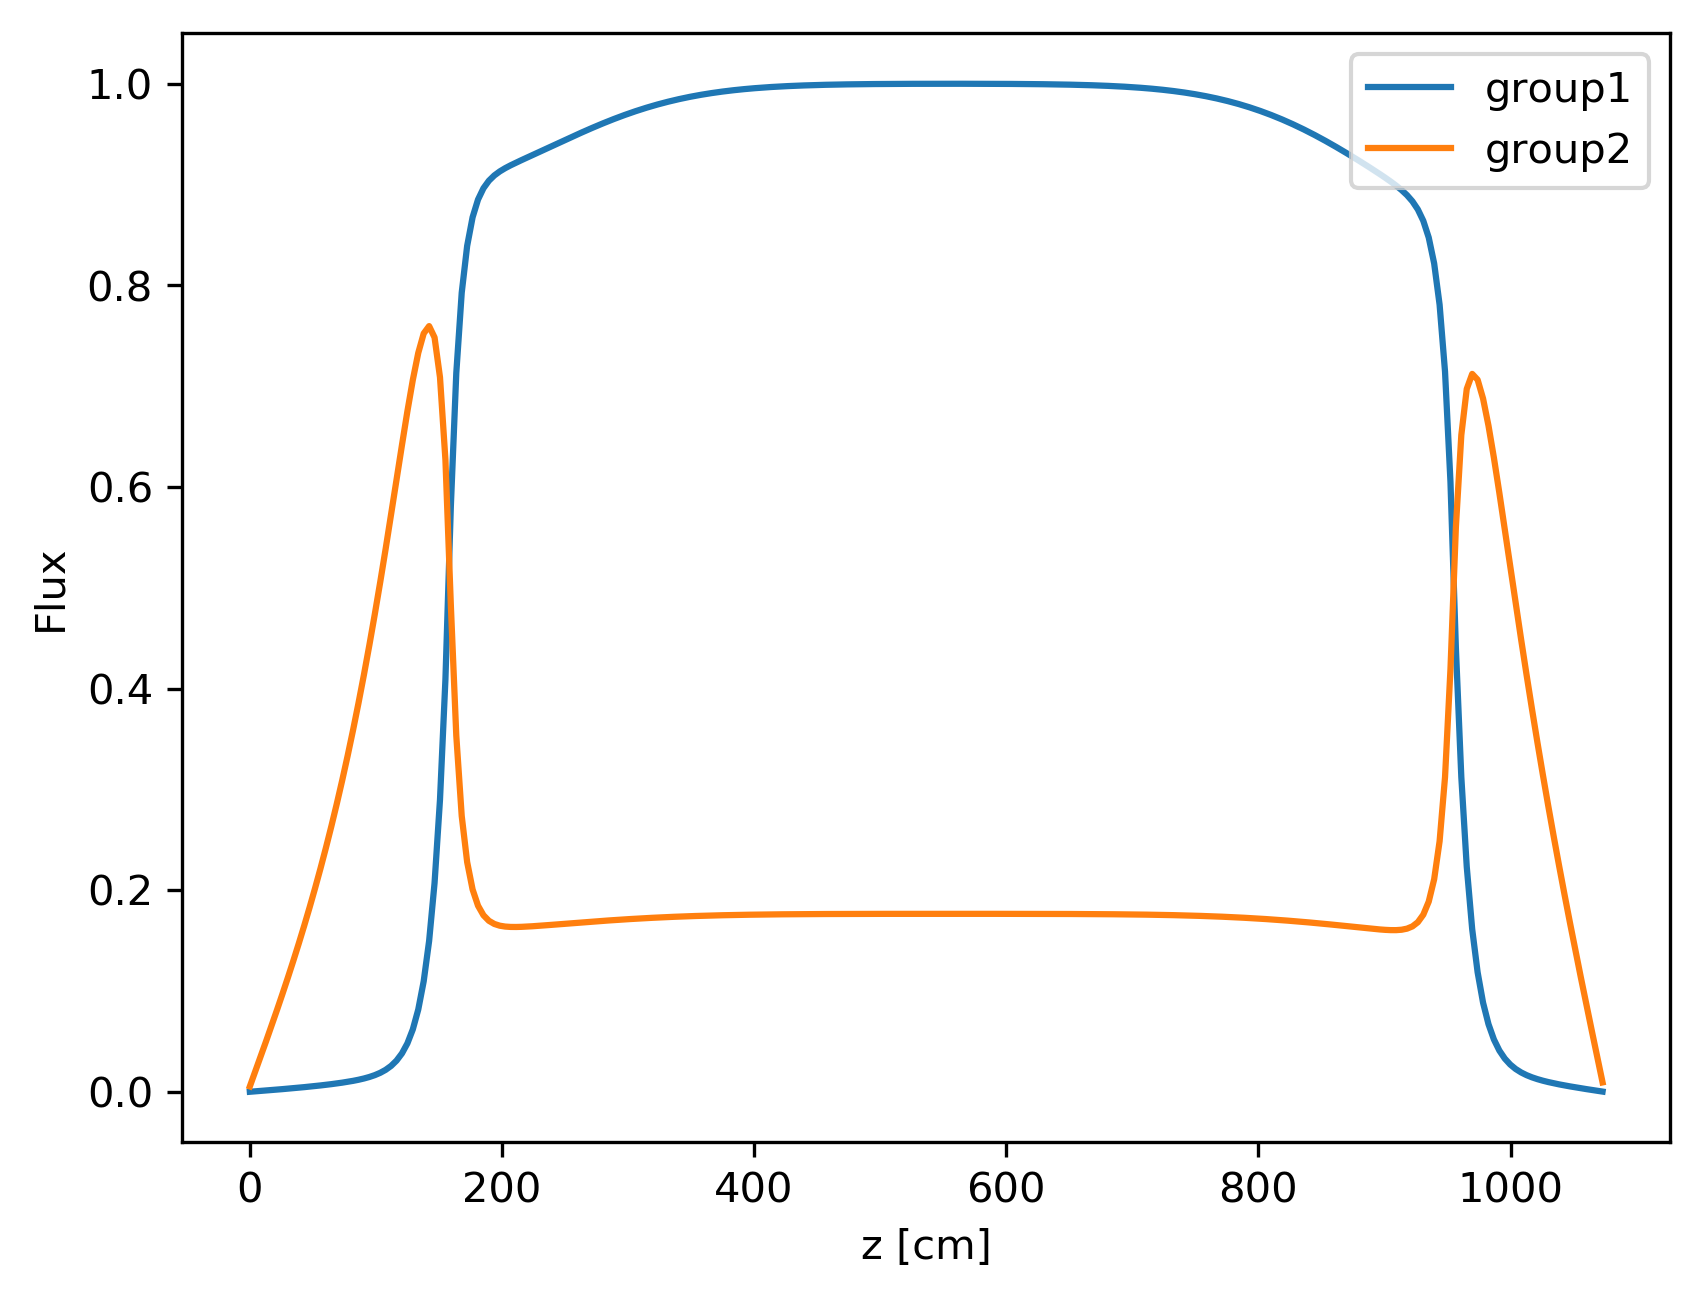
\includegraphics[width=\linewidth]{1D-fuel-reflec-eig1B}
			\caption{Inverse Power Method.}
		\end{subfigure}
		\begin{subfigure}[t]{0.4\textwidth}
			\centering
			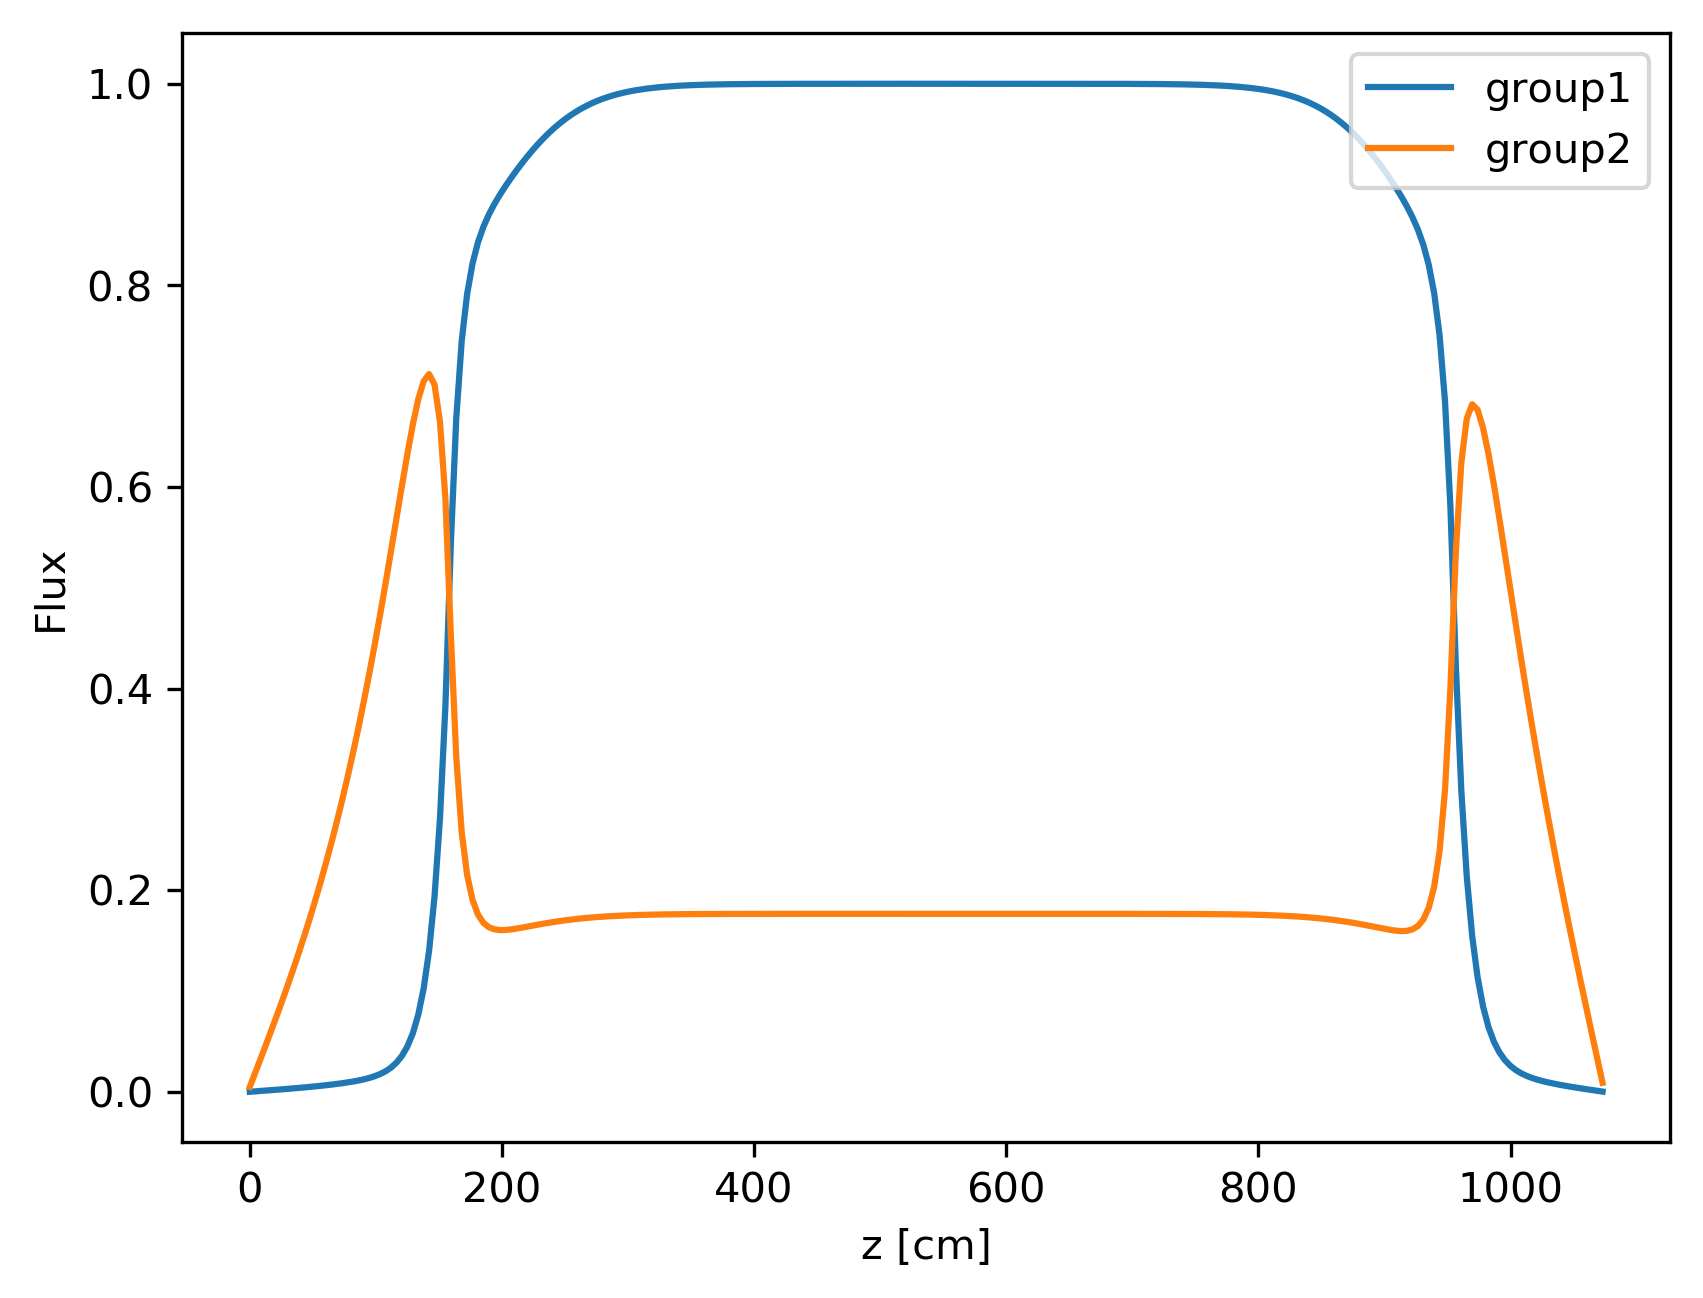
\includegraphics[width=\linewidth]{1D-fuel-reflec-eig2B}
			\caption{Non Linear Eigen.}
		\end{subfigure}
		\hfill
		\caption{Steady state Group 1 and 2 fluxes for different eigenvalue iteration methods.}
		\label{fig:1D-fuel-reflec-eig2}
	\end{figure}

\pagebreak
\bibliographystyle{plain}
% \bibliography{bibliography}

\end{document}
